\documentclass{beamer}
\mode<presentation>
\usetheme{CambridgeUS}
\usepackage[russian]{babel}
\usepackage[utf8]{inputenc}
\usepackage[T2A]{fontenc}
\usepackage{sansmathaccent}

\usepackage{verbatim}
\usepackage{alltt}

\pdfmapfile{+sansmathaccent.map}
\title[UX Elements]{Функциональные спецификации и требования к контенту}
\author{Наумов Д.А., доц. каф. КТ}
\date[23.09.2020] {Компьютерная графика и проектирование графических интерфейсов, 2020}

\begin{document}

%ТИТУЛЬНЫЙ СЛАЙД
\begin{frame}
  \titlepage
\end{frame}
  
%СОДЕРЖАНИЕ ЛЕКЦИИ
\begin{frame}
  \frametitle{Содержание лекции}
  \tableofcontents  
\end{frame}

\section{Уровень набора возможностей}
  
\begin{frame}[t]
\begin{block}{Определение набора возможностей}
представляет ценность
\begin{itemize}
\item как процесс -- заставляет выявлять потенциальные противоречия и <<шероховатости>> конечного продукта на том этапе, когда сам результат существует лишь в вашей голове;
\item как результат -- дает точку отсчета для всей последующей работы над проектом и общий язык, на котором вы сможете обсуждать эту работу. 
\end{itemize}
\end{block}
\begin{figure}[h]
\centering
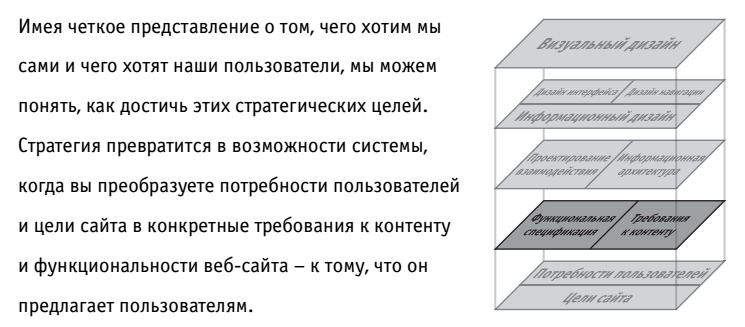
\includegraphics[scale=0.4]{images/lec02-pic01.png}
\end{figure}
\end{frame} 

\begin{frame}[t]
Необходимость описания набора возможностей:
\begin{enumerate}
\item вы будете знать, что именно вы создаете;
\item вы будете знать, что именно вы не создаете;
\item вы будете знать, что именно вы не создаете прямо сейчас;
\end{enumerate}
\begin{figure}[h]
\centering
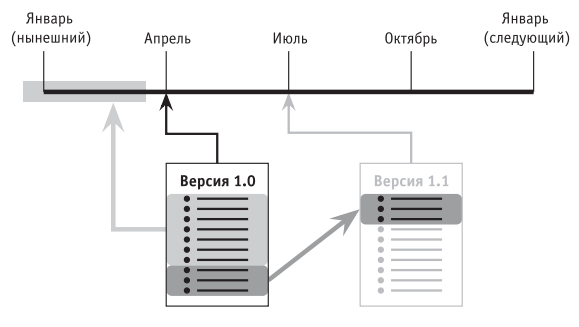
\includegraphics[scale=0.5]{images/lec02-pic02.png}
\end{figure}
\end{frame}  

\begin{frame}[t]{Функциональность и контент}
Набор возможностей определяется в документах, содержащих требования к функциональности, или в \textbf{функциональных спецификациях}.
\begin{figure}[h]
\centering
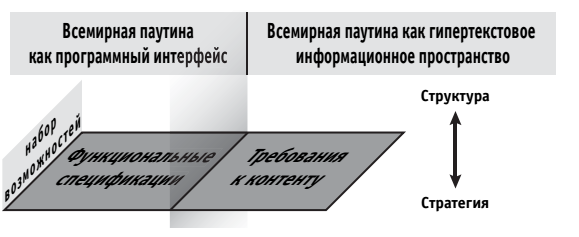
\includegraphics[scale=0.5]{images/lec02-pic03.png}
\end{figure}
При \textbf{разработке контента }определение требований часто не включается в формальную процедуру.
\end{frame} 

\begin{frame}[t]
\begin{figure}[h]
\centering
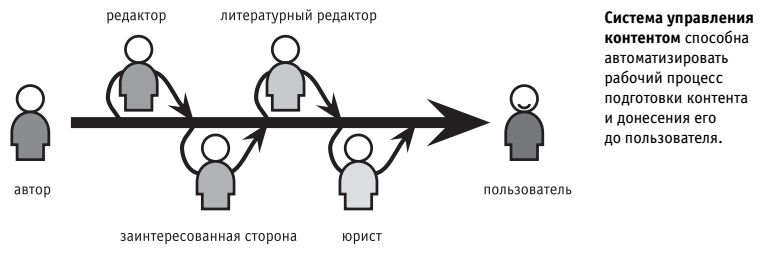
\includegraphics[scale=0.5]{images/lec02-pic04.png}
\end{figure}
\begin{itemize}
\item Функциональность зависит от природы самого контента. 
	\begin{itemize}
	\item Нужно ли вам поддерживать несколько языков и различные форматы данных? 
	\item Должен ли каждый пресс-релиз визироваться юристом? 
	\item Будут ли элементы содержимого сайта автоматически переупорядочиваться в соответствии с предпочтениями каждого пользователя? 	
	\end{itemize}
\item Функциональные требования влияют на контент.
	\begin{itemize}
	\item Потребуются ли инструкции на экране настроек?
	\item Как насчет сообщений об ошибках?
	\end{itemize}
\end{itemize}
\end{frame}

\begin{frame}[t]{Требования к контенту}
\begin{itemize}
\item количество слов текста (в статье);
\item размеры изображений в пикселях;
\item размеры отдельных скачиваемых файлов (PDF-документов, аудио- и видеофайлов);
\item кто из сотрудников за какой элемент контента отвечает?
\item как часто элемент контента он будет обновляться?
\end{itemize}
\end{frame}

\section{Анализ требований}

\begin{frame}[t]{Понятие анализа требований}
\begin{figure}[h]
\centering
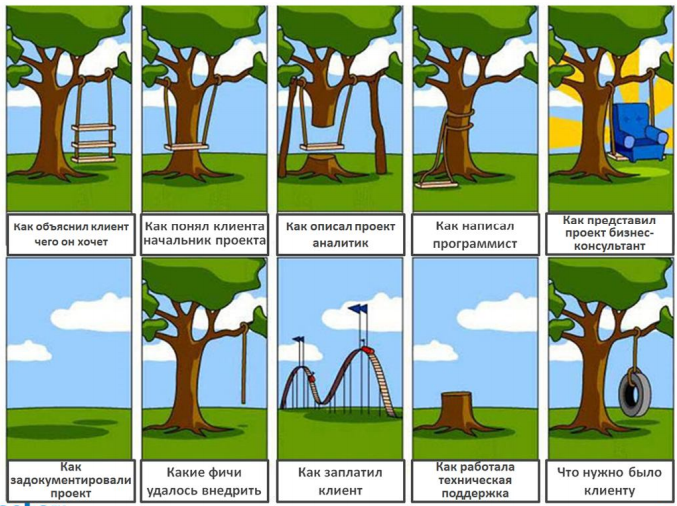
\includegraphics[scale=0.5]{images/lec02-pic06.png}
\end{figure}
\end{frame} 

\begin{frame}[t]{Понятие анализа требований}
\begin{figure}[h]
\centering
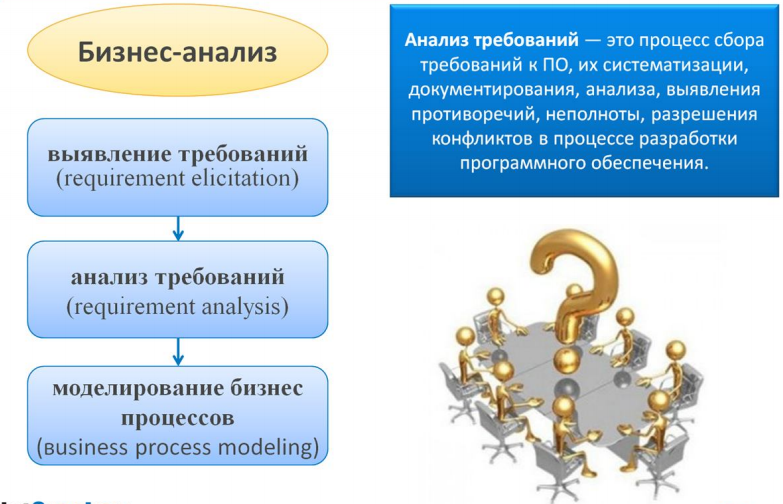
\includegraphics[scale=0.5]{images/lec02-pic07.png}
\end{figure}
\end{frame} 

\begin{frame}[t]{Структура анализа требований}
\begin{figure}[h]
\centering
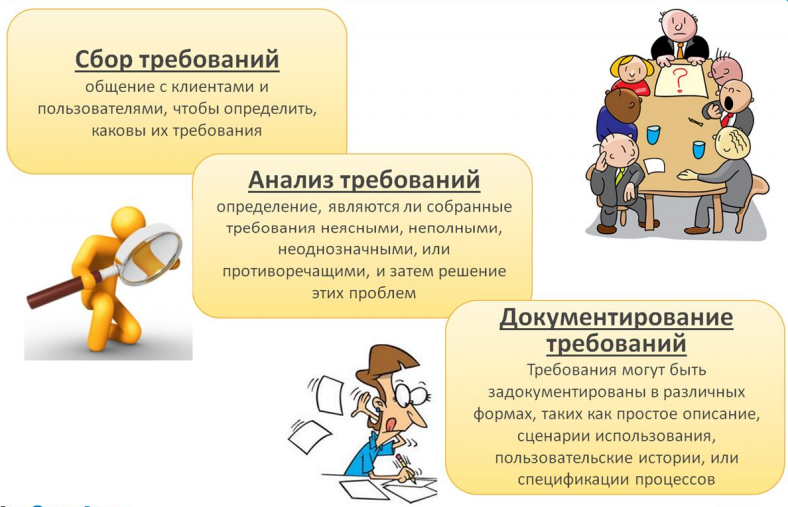
\includegraphics[scale=0.5]{images/lec02-pic08.png}
\end{figure}
\end{frame}

\begin{frame}[t]{Виды требований по характеру}
\begin{figure}[h]
\centering
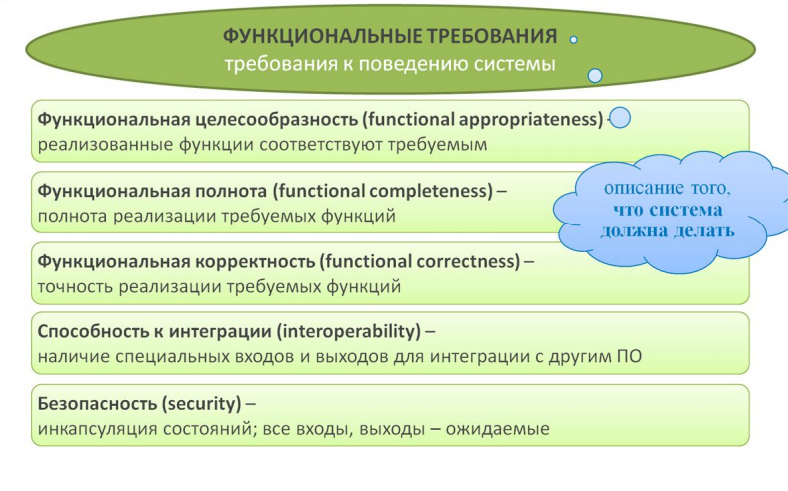
\includegraphics[scale=0.5]{images/lec02-pic09.png}
\end{figure}
\end{frame}    

\begin{frame}[t]{Виды требований по характеру}
\begin{figure}[h]
\centering
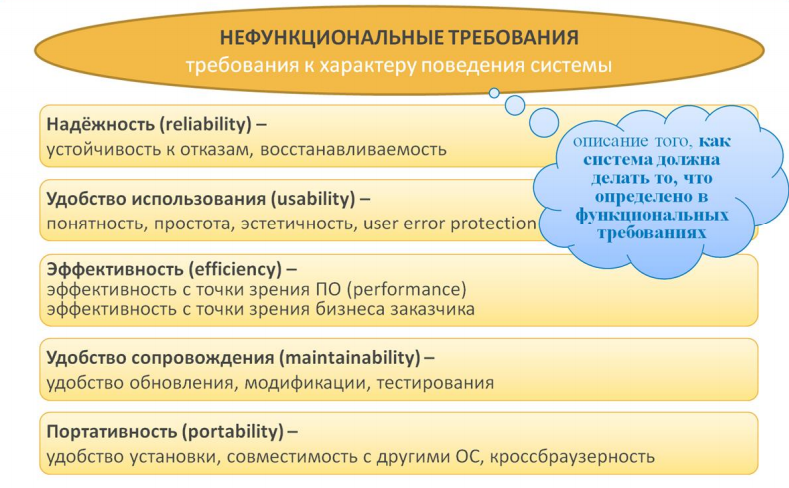
\includegraphics[scale=0.5]{images/lec02-pic10.png}
\end{figure}
\end{frame}    

\begin{frame}[t]{Трассировка требований}
\begin{figure}[h]
\centering
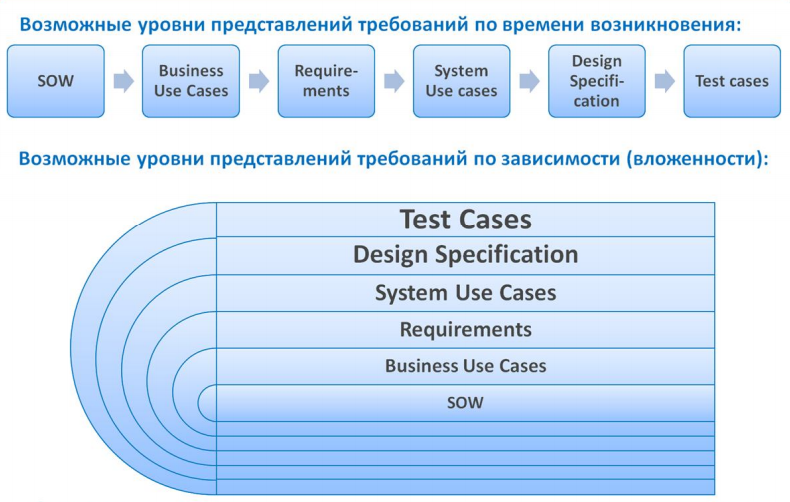
\includegraphics[scale=0.5]{images/lec02-pic11.png}
\end{figure}
\end{frame}    

\begin{frame}[t]{Трассировка требований}
\begin{itemize}
\item SOW – Statement of Work, требования высокого уровня, наимение конкретные, без четкой детализации.
\item Business Use Cases – варианты использования (Use Case) на уровне бизнеса
\item Requirements – список требований, разделенные на функциональные, нефункциональные и т.п. Структурированный документ.
\item System Use Cases – варианты использования (Use Case) на уровне ПО Design Specification – проектная спецификация, техзадание (для разработчиков).
\item Test Cases – варианты использования готового ПО, соответствия реального поведения и желаемого. Наиболее формализованные требования.
\end{itemize}
\end{frame}

\begin{frame}[t]{Методы выявления требований}
\begin{figure}[h]
\centering
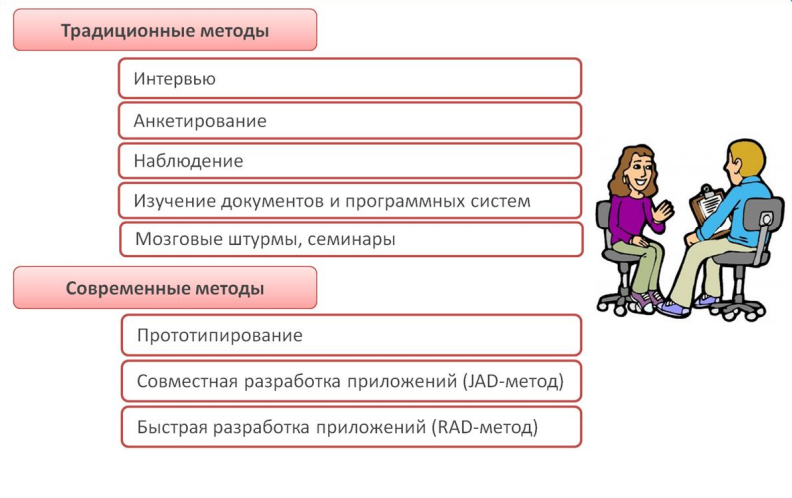
\includegraphics[scale=0.5]{images/lec02-pic12.png}
\end{figure}
\end{frame}

\begin{frame}[t]{Характеристики качественных требований}
\begin{figure}[h]
\centering
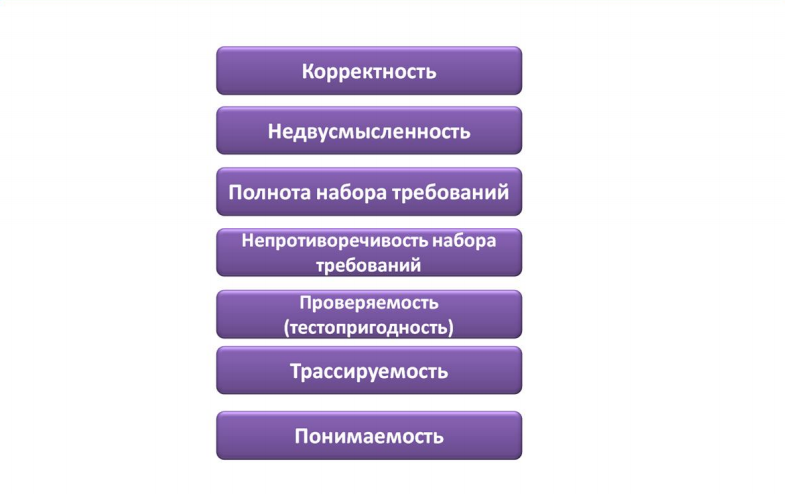
\includegraphics[scale=0.5]{images/lec02-pic13.png}
\end{figure}
\end{frame}

\begin{frame}[t]{Корректность}
Насколько корректно наше требование? Действительно ли это то, что требуется от
системы или кто-то допустил ошибку/опечатку в процессе написания требования?

\textbf{Пример}: после набора номера пользователь должен слышать короткие гудки (символизирующие о том,
что идет дозвон)

\textbf{Описание}: просто перепутали слово. Гудки должны быть длинными.

Как тестировать на корректность и находить такие ошибки:
\begin{itemize}
\item нужны хорошие доменные знания в области 
\item нужно смотреть на трассировку вверх и вниз, возможно обнаружится нестыковка и будет зацепка;
\item процесс ревью также может помочь (желательно, чтобы это ревью проводил;
тест-аналитик или тот, кто тоже имеет отношение к написанию требований.
\end{itemize}
\end{frame}

\begin{frame}[t]{Недвусмысленность}
Могут ли 2 различных человека понять требование по-разному?

\textbf{Пример}: Телефон должен работать в автономном режиме, когда он питается от батареек. В
автономном режиме недоступны следующие функции: бла-бла-бла.

\textbf{Описание}: должны ли быть доступны функции «бла-бла-бла», если телефон с батарейками, но подключен к
сети? Я могу подумать, что да, программист — что нет. Заказчик тоже может это интерпретировать как захочет

Как тестировать на корректность и находить такие ошибки:
\begin{itemize}
\item Проверять «ветвистость» требований
\item Ревью, аналогично предыдущему пункту
\item В идеале — стараться избегать ветвлений в требованиях. Если это невозможно — форматировать их в виде
таблиц со всеми возможными вариантами.
\end{itemize}
\end{frame}

\begin{frame}[t]{Полнота набора требований}
Насколько полным является набор требований? Если есть секция в SRS, определяющая функциональность
модуля, то вся ли функциональность этого модуля покрыта требованиями? Нет ли дыр?

\textbf{Пример}: Есть секция требований, определяющая работу со спец-кнопками, и в этих
требованиях упущена из виду одна из спец-кнопок. Для этой кнопки просто нет требований.

Как тестировать на корректность и находить такие ошибки:
\begin{itemize}
\item нужно смотреть на трассировку требований вверх и вниз (на бизнес-требования и на низкоуровневые
требования — дизайн, макеты, детальное описание реализации). 
\item Если в этих требованиях есть то, что упущено в SRS — такая ошибка сразу обнаружится. 
\item Если этого и там нет — то, возможно, этой функциональности и не должно быть? Или должна быть, но она упущена из виду во всех документах
\end{itemize}
\end{frame}

\begin{frame}[t]{Непротиворечивость набора требований }
Поиск требований, которые противоречат друг другу. 

\textbf{Пример}: 

\textit{Требование 1} (из раздела функциональности спец-кнопок): когда активен режим «Mute», телефон не должен издавать никаких звуков

\textit{Требование 245} (из раздела интерфейса): когда пользователь снимает трубку, телефон должен издавать тоновые гудки

Как тестировать на корректность и находить такие ошибки:
\begin{itemize}
\item обращать внимания на общие формулировки в требованиях; 
\item делить на категории (например, выделить все требования, регламентирующие
звуковые сигналы) и ревьювить их направленно на предмет противоречий;
\item выделять все требования, трассирующиеся на одно верхнеуровневое требование
и анализировать такие наборы. 
\end{itemize}
\end{frame}

\begin{frame}[t]{Проверяемость (тестопригодность)}
Один из основных и самых важных критериев (для QA инженеров). Возможно ли проверить это требование и убедиться, что оно выполняется?

\textbf{Пример}: в случае возникновения критической ошибки телефон должен
перезагрузиться

\textbf{Пример 2}: информация на дисплее телефона должна отображаться в понятном
пользователю виде

Как тестировать на корректность и находить такие ошибки:
\begin{itemize}
\item Во время анализа требований задавать вопрос: «Как я буду это проверять?». Если
однозначного ответа нет — значит нужно более детально анализировать, и,
возможно, вносить правки в требование (уточнения, ограничения)
\item Во время анализа требований выявлять общие формулировки, требующие
перебора неопределенного числа вариантов для проверки выполнения
требования.
\end{itemize}
\end{frame}

\begin{frame}[t]{Трассируемость}
\textbf{Трассируемость} — это связь с требованием выше и требованием ниже.

\textbf{Пример 1}. Бизнес-требование не имеет ни одного SRS требования. Соответственно, получается
пробел в реализации (мы не сделаем того, что нужно бизнесу)

\textbf{Пример 2}. SRS требование описывает то, чего не было в бизнес-требованиях. Получается, мы
делаем то, что не требовалось.

Как тестировать на корректность и находить такие ошибки:
\begin{itemize}
\item если используется какая-то система менеджмента требований — то там, скорее
всего, уже есть функциональность, позволяющая в автоматическом режиме
следить за трассировкой
\item если системы менеджмента требований нет, то остается "дедовский" способ —
составлять матрицы трассируемости и отслеживать связи всех
требований на всех уровнях. 
\end{itemize}
\end{frame}

\begin{frame}[t]{Понимаемость}
Могут ли все участники процесса понять, что требуется от системы по описанию
требования? Часто бывают ситуации, когда требование может быть понятно разработчику, но не
понятно тестировщику (или наоборот). При этом требование может вполне
соответствовать остальным критериям.

\textbf{Пример}: передатчик телефона должен использовать амплитудно-фазовую
модуляцию с несущими от 2 до 7,5 МГц с шагом 500 кГц

Как тестировать на корректность и находить такие ошибки:
\begin{itemize}
\item стараться представлять себя на месте заказчика/аналитика/простого
пользователя и пытаться представить, будет ли понятно это требование;
\item обращать внимание на двойственные термины (особенно, аббревиатуры),
которые могут интерпретироваться по-разному различными людьми. 
\end{itemize}
\end{frame}

\begin{frame}[t]{Критерии формулировки требований}
\begin{figure}[h]
\centering
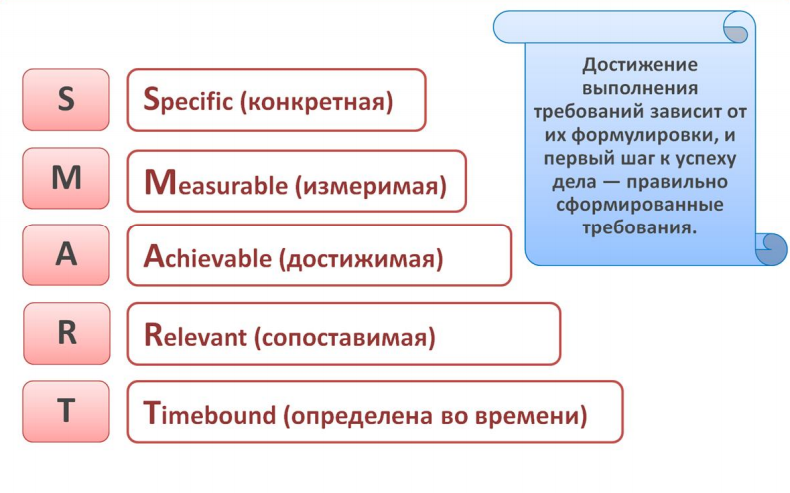
\includegraphics[scale=0.5]{images/lec02-pic14.png}
\end{figure}
\end{frame}

\end{document}
